\documentclass{article}\usepackage[]{graphicx}\usepackage[]{color}
%% maxwidth is the original width if it is less than linewidth
%% otherwise use linewidth (to make sure the graphics do not exceed the margin)
\makeatletter
\def\maxwidth{ %
  \ifdim\Gin@nat@width>\linewidth
    \linewidth
  \else
    \Gin@nat@width
  \fi
}
\makeatother

\definecolor{fgcolor}{rgb}{0.345, 0.345, 0.345}
\newcommand{\hlnum}[1]{\textcolor[rgb]{0.686,0.059,0.569}{#1}}%
\newcommand{\hlstr}[1]{\textcolor[rgb]{0.192,0.494,0.8}{#1}}%
\newcommand{\hlcom}[1]{\textcolor[rgb]{0.678,0.584,0.686}{\textit{#1}}}%
\newcommand{\hlopt}[1]{\textcolor[rgb]{0,0,0}{#1}}%
\newcommand{\hlstd}[1]{\textcolor[rgb]{0.345,0.345,0.345}{#1}}%
\newcommand{\hlkwa}[1]{\textcolor[rgb]{0.161,0.373,0.58}{\textbf{#1}}}%
\newcommand{\hlkwb}[1]{\textcolor[rgb]{0.69,0.353,0.396}{#1}}%
\newcommand{\hlkwc}[1]{\textcolor[rgb]{0.333,0.667,0.333}{#1}}%
\newcommand{\hlkwd}[1]{\textcolor[rgb]{0.737,0.353,0.396}{\textbf{#1}}}%

\usepackage{framed}
\makeatletter
\newenvironment{kframe}{%
 \def\at@end@of@kframe{}%
 \ifinner\ifhmode%
  \def\at@end@of@kframe{\end{minipage}}%
  \begin{minipage}{\columnwidth}%
 \fi\fi%
 \def\FrameCommand##1{\hskip\@totalleftmargin \hskip-\fboxsep
 \colorbox{shadecolor}{##1}\hskip-\fboxsep
     % There is no \\@totalrightmargin, so:
     \hskip-\linewidth \hskip-\@totalleftmargin \hskip\columnwidth}%
 \MakeFramed {\advance\hsize-\width
   \@totalleftmargin\z@ \linewidth\hsize
   \@setminipage}}%
 {\par\unskip\endMakeFramed%
 \at@end@of@kframe}
\makeatother

\definecolor{shadecolor}{rgb}{.97, .97, .97}
\definecolor{messagecolor}{rgb}{0, 0, 0}
\definecolor{warningcolor}{rgb}{1, 0, 1}
\definecolor{errorcolor}{rgb}{1, 0, 0}
\newenvironment{knitrout}{}{} % an empty environment to be redefined in TeX

\usepackage{alltt}
\usepackage[utf8]{inputenc}
\usepackage[hmargin=2cm,vmargin=1.5cm,bmargin=1.5cm]{geometry}
\title{Análise estatística de dados com objetivo de identificar clientes propensos a cancelar produtos de um banco}
\author{Daniel V. F. Falbel}
\date{16 de Novembro de 2014}
\IfFileExists{upquote.sty}{\usepackage{upquote}}{}
\begin{document}
\maketitle

\section*{Resumo}

Para auxiliar um banco na criação de ações publicitárias para retenção de clientes que possuem um certo cartão de crédito, este trabalho apresenta uma análise estatística que permite a identificação dos clientes mais propensos a cancelar o produto.

\section{Descrição do problema}

Um banco deseja fazer ações de marketing para reter os seus clientes, evitar que eles cancelem seus produtos. Para poder fazer ações mais acertivas, o banco deseja saber qual é o perfil dos clientes com maior propensão a cancelar um certo cartão de crédito.

As variáveis que podem ajudar na identificação dos perfis estão listadas abaixo: 

\begin{itemize}
  \item sexo: M-masculino; F-feminino
  \item modulo: Segmentação de clientes; valores mais baixos representam clientes com menor renda ou investimento, valores mais altos representam clientes mais interessantes para a instituição
  \item cheque: Classificação da conta corrente; quanto maior o valor, mais "especial" o cliente
  \item evolcredor: Evolução do saldo credor médio trimestral (A: aumentou, D: diminuiu, M: manteve)
  \item evoldevedor: Evolução do saldo devedor médio trimestral (A: aumentou, D: diminuiu, M: manteve)
  \item evolpoup:  do saldo da poupança trimestral (A: aumentou, D: diminuiu, M: manteve)
  \item idade: idade em anos
  \item salario: está categorizado em 10 categorias (quanto maior, maior o salário)
  \item cartaocancel: Cancelamento do cartão de credito pelo banco 0 - não cancelou; 1 - cancelou
  \item bancsal: 0: não recebe salário pelo banco; 1: recebe salário pelo banco
  \item tempo: Tempo de permanência com um determinado produto, em meses
  \item status: 1: tempo refere-se ao tempo da contratação até o cancelamento do produto; 0: tempo da contratação até término de acompanhamento sem cancelamento (censura)
\end{itemize}

\section{Análise Descritiva}



Para verificar se existem possíveis inconsistências nos dados, foi feita uma análise exploratória. Além disso, podemos já ter uma ideia do que pode influencia no tempo até o cancelamento do cartão de crédito. 

\begin{figure}
\centering
\begin{knitrout}
\definecolor{shadecolor}{rgb}{0.969, 0.969, 0.969}\color{fgcolor}
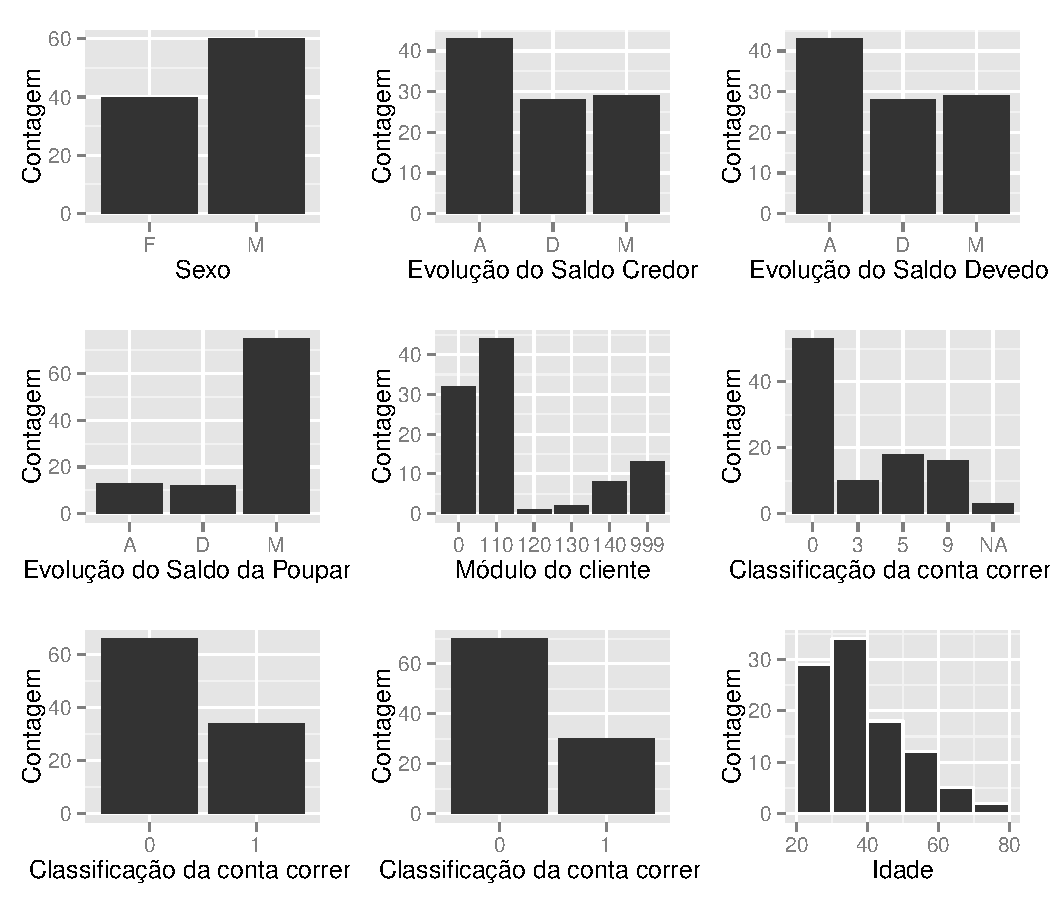
\includegraphics[width=\maxwidth]{figure/unnamed-chunk-2} 

\end{knitrout}
\caption{(i) quantidade de clientes em cada categoria da variável sexo, (ii) quantidade de clientes em cada categoria de evolução do saldo credor, (iii) quantidade de clientes em cada categoria de evolução do saldo devedor, (iv) quantidade de clientes em cada categoria de evolução do saldo da poupança, (v) quantidade de clientes em cada módulo (segmento) criado pelo banco, (vi) quantidade de clientes em  cada classificação da conta corrente, (vii) quantidade de clientes que cancelaram o cartão (1), (viii) quantidade de clientes que recebem o salário por meio do banco, (ix) histograma da idade dos clientes}
\end{figure}

Pelos gráficos da figura 1, podemos observar que 60\% dos clientes são do sexo masculino. A maior parte dos clientes teve um aumento do saldo credor e do saldo devedor. Também podemos analisar que a maior parte dos clientes manteve estável o saldo da poupança. Observamos que a maior parte dos clienes estão no segmento 110 do módulo, e que cerca de 50\% dos cliente estão na classificação 0 da conta corrente. Note que no gráfico (vi) existe a ocorrência de uma observação ausente, isto é, não temos a informação de que tipo de conta o cliente ppossui.

\begin{figure}[t!]

\centering
\begin{knitrout}
\definecolor{shadecolor}{rgb}{0.969, 0.969, 0.969}\color{fgcolor}
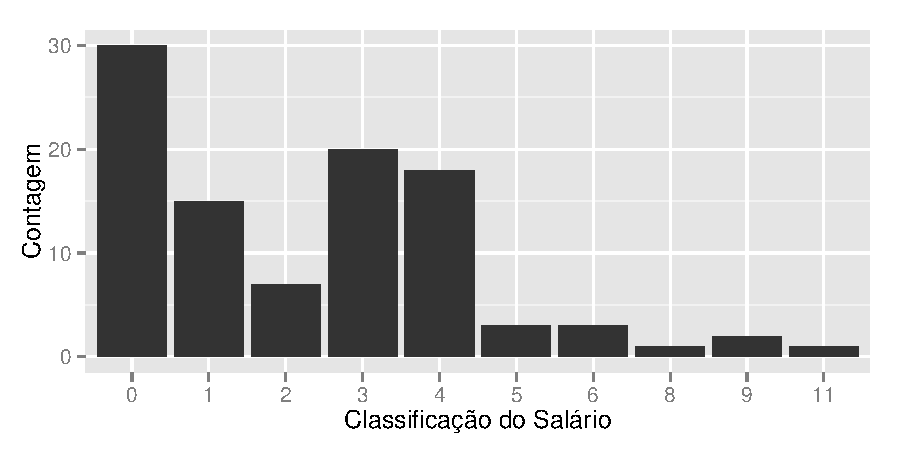
\includegraphics[width=\maxwidth]{figure/unnamed-chunk-3} 

\end{knitrout}
\caption{Quantidade de clientes em cada classificação do salário}
\end{figure}

Pela figura 2 observamos que cerca de 30\% dos clientes ganham até R\$300,00, em seguida as categorias com mais indivíduos são a 3 e a 4 que contém pessoas que ganham de R\$501,00 a R\$1500,00.

\begin{figure}[t!]

\centering
\begin{knitrout}
\definecolor{shadecolor}{rgb}{0.969, 0.969, 0.969}\color{fgcolor}
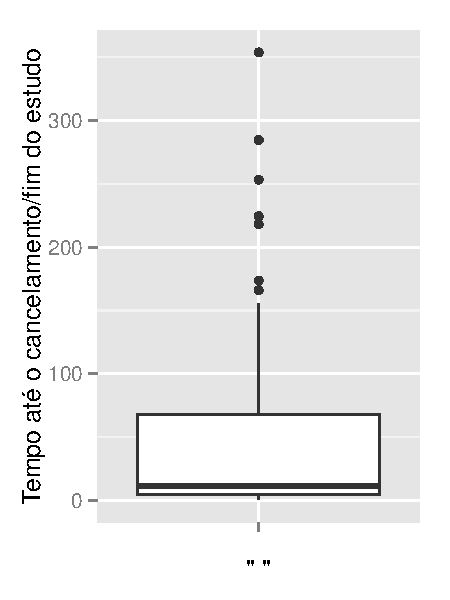
\includegraphics[width=\maxwidth]{figure/unnamed-chunk-4} 

\end{knitrout}
\caption{Boxplot do tempo até o cancelamento do cartão de crédito ou fim do acompanhamento}
\end{figure}

Na figura 3, vemos que os clientes em mediana têm o produto por 11 meses. Aproximadamente 75\% dos clientes tem tempo até 68 meses. O indivíduo que possui o produto a mais tempo, o tem a 353 meses. No estudo observamos que 18 clientes foram censurados, ou seja, ainda não tinham cancelado o cartão de crédito até a data de fim do acompanhamento.












\end{document}
